% Source: graduate-coursework/Research/Intro_to_Agents/handouts/Part2_Agent_Foundations.tex

\documentclass[border=4pt]{standalone}
\usepackage{amsmath}
\usepackage{amssymb}
\usepackage{tikz}
\usepackage{xcolor}
\usetikzlibrary{shapes.geometric, arrows.meta, positioning, fit, calc, backgrounds}

\definecolor{UofSCGarnet}{HTML}{73000a}
\definecolor{UofSCBlack}{HTML}{000000}
\definecolor{UofSCWhite}{HTML}{ffffff}
\definecolor{UofSCAtlantic}{HTML}{466A9F}
\definecolor{UofSCCongaree}{HTML}{1F414D}
\definecolor{UofSCRose}{HTML}{CC2E40}
\definecolor{UofSCHorseshoe}{HTML}{65780B}
\definecolor{UofSCGrass}{HTML}{CED318}
\definecolor{UofSCHoneycomb}{HTML}{A49137}
\definecolor{UofSCDarkGarnet}{HTML}{570008}
\definecolor{UofSCAzalea}{HTML}{844247}
\definecolor{UofSC90Black}{HTML}{363636}
\definecolor{UofSC70Black}{HTML}{5C5C5C}
\definecolor{UofSC50Black}{HTML}{A2A2A2}
\definecolor{UofSCWarmGrey}{HTML}{676156}
\definecolor{UofSCSandstorm}{HTML}{FFF2E3}

\tikzset{
    % Box styles with sharp corners
    component/.style={
        rectangle,
        draw=UofSCBlack,
        fill=UofSCWhite,
        thick,
        minimum width=3cm,
        minimum height=1cm,
        align=center,
        font=\small
    },
    component garnet/.style={
        component,
        fill=UofSCGarnet!10,
        draw=UofSCGarnet,
        thick
    },
    component atlantic/.style={
        component,
        fill=UofSCAtlantic!10,
        draw=UofSCAtlantic,
        thick
    },
    component congaree/.style={
        component,
        fill=UofSCCongaree!10,
        draw=UofSCCongaree,
        thick
    },
    loop node/.style={
        rectangle,
        draw=UofSCGarnet,
        fill=UofSCGarnet!15,
        thick,
        minimum width=2.5cm,
        minimum height=1.2cm,
        align=center,
        font=\footnotesize\bfseries
    },
    decision/.style={
        diamond,
        draw=UofSCBlack,
        fill=UofSCHoneycomb!20,
        thick,
        minimum width=2cm,
        minimum height=1.5cm,
        align=center,
        font=\footnotesize,
        aspect=2
    },
    arrow style/.style={
        ->,
        >=Stealth,
        thick,
        UofSCBlack
    },
    biarrow style/.style={
        <->,
        >=Stealth,
        thick,
        UofSCBlack
    }
}

\begin{document}
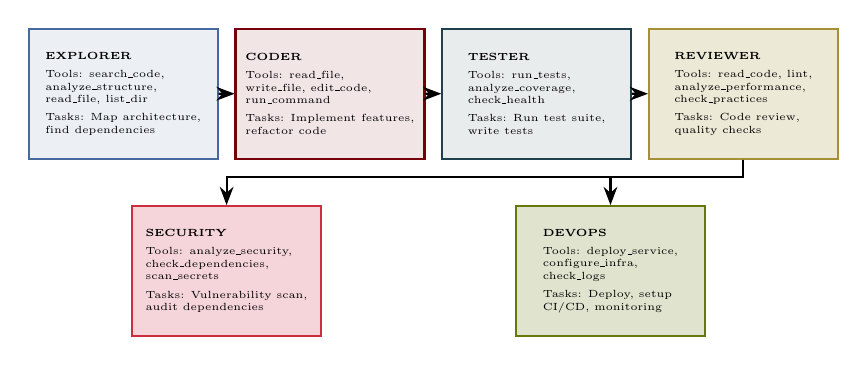
\begin{tikzpicture}[scale=0.75, transform shape]
        % Explorer
        \node[component atlantic, minimum width=3.2cm, minimum height=2.2cm, align=left, font=\tiny] (explorer) at (-5, 1.5) {
            \textbf{EXPLORER}\\[0.1cm]
            Tools: search\_code,\\
            analyze\_structure,\\
            read\_file, list\_dir\\[0.1cm]
            Tasks: Map architecture,\\
            find dependencies
        };

        % Coder
        \node[component garnet, minimum width=3.2cm, minimum height=2.2cm, align=left, font=\tiny] (coder) at (-1.5, 1.5) {
            \textbf{CODER}\\[0.1cm]
            Tools: read\_file,\\
            write\_file, edit\_code,\\
            run\_command\\[0.1cm]
            Tasks: Implement features,\\
            refactor code
        };

        % Tester
        \node[component congaree, minimum width=3.2cm, minimum height=2.2cm, align=left, font=\tiny] (tester) at (2, 1.5) {
            \textbf{TESTER}\\[0.1cm]
            Tools: run\_tests,\\
            analyze\_coverage,\\
            check\_health\\[0.1cm]
            Tasks: Run test suite,\\
            write tests
        };

        % Reviewer
        \node[component, fill=UofSCHoneycomb!20, draw=UofSCHoneycomb, minimum width=3.2cm, minimum height=2.2cm, align=left, font=\tiny] (reviewer) at (5.5, 1.5) {
            \textbf{REVIEWER}\\[0.1cm]
            Tools: read\_code, lint,\\
            analyze\_performance,\\
            check\_practices\\[0.1cm]
            Tasks: Code review,\\
            quality checks
        };

        % Security
        \node[component, fill=UofSCRose!20, draw=UofSCRose, minimum width=3.2cm, minimum height=2.2cm, align=left, font=\tiny] (security) at (-3.25, -1.5) {
            \textbf{SECURITY}\\[0.1cm]
            Tools: analyze\_security,\\
            check\_dependencies,\\
            scan\_secrets\\[0.1cm]
            Tasks: Vulnerability scan,\\
            audit dependencies
        };

        % DevOps
        \node[component, fill=UofSCHorseshoe!20, draw=UofSCHorseshoe, minimum width=3.2cm, minimum height=2.2cm, align=left, font=\tiny] (devops) at (3.25, -1.5) {
            \textbf{DEVOPS}\\[0.1cm]
            Tools: deploy\_service,\\
            configure\_infra,\\
            check\_logs\\[0.1cm]
            Tasks: Deploy, setup\\
            CI/CD, monitoring
        };

        % Pipeline arrows
        \draw[arrow style] (explorer) -- (coder);
        \draw[arrow style] (coder) -- (tester);
        \draw[arrow style] (tester) -- (reviewer);
        \draw[arrow style] (reviewer.south) -- ++(0,-0.3) -| (security.north);
        \draw[arrow style] (reviewer.south) -- ++(0,-0.3) -| (devops.north);
    \end{tikzpicture}
\end{document}
